\documentclass{article}

\usepackage{graphicx}
\usepackage{hyperref}
\usepackage{bm}
\usepackage{float}
\restylefloat{table}

\usepackage{listings}
\usepackage{color}
\usepackage{amsmath}

\usepackage[margin=1.25in]{geometry}

\definecolor{dkgreen}{rgb}{0,0.6,0}
\definecolor{gray}{rgb}{0.5,0.5,0.5}
\definecolor{mauve}{rgb}{0.86,0.27,0.22}

\lstset{frame=tb,
  language=python,
  aboveskip=3mm,
  belowskip=3mm,
  showstringspaces=false,
  columns=flexible,
  basicstyle={\small\ttfamily},
  numbers=left,
  stepnumber=1,
  numberstyle=\tiny\color{gray},
  keywordstyle=\color{blue},
  commentstyle=\color{dkgreen},
  stringstyle=\color{mauve},
  breaklines=true,
  breakatwhitespace=true,
  tabsize=3
}

\title{CS5200: Prelim Exam \#2} % Title of the assignment

\author{Matthew Whitesides\\ \texttt{mbwxd4@umsystem.edu}} % Author name and email address

\date{\today} % University, school and/or department name(s) and a date

%----------------------------------------------------------------------------------------

\begin{document}

  \maketitle % Print the title

  \textit{I, Matthew Whitesides, certify that all the material in this PDF file is my original work, that I did not discuss these questions with anyone other than my instructor, and that I did not copy work from anyone for this examination.}
 
  \begin{enumerate}
    \item \textbf{Probability}.
    
    First let's setup our sample space. Given that it dosen't really matter what disk we change lets say disk one stays the same and we place disk two on top and rotate it.

    Disk two will have 128 possible differnt positions it can be placed on top of disk one. Therefore:
    
    \[S=\{1,2,...,128\}\]

    Now let's define for each $i$ in the sammple space $S$, we have a $j$ meaning if $i = 1$ that sector 1 of the second disk is placed ontop of sector $j$ of the first disk.

    Next let's define a random variable $S\rightarrow R$ given by Matches(j) = the number of matches when disk two's slice 1 is over disk one's slick $j$.

    Now since we have a sample space of 128 we'll need to calculate the matches for each sector using indicator variables.\\

    Let's define $M_i:S\rightarrow R$ meaning matches given sample space i given by:

    $M_i(j) = 1$ If sector $i$ of disk two has a match over disk one's sector $j$.

    $M_i(j) = 0$ If no match.

    Therefore the total matches would be the sum of each indicator variable:

    \[\sum_{i=1}^{128}E(M_i)\]

    Now we just need to calcualte the chance there's a match or no match for any given sector.

    Our possibile probability for each sector are (position one being color of disk one and two being two) with RR, WW being matches and RW, WR being not:

    \[\{RR, RW, WR, WW\} = \{\frac{1}{4} \frac{1}{2}, \frac{1}{4} \frac{1}{2}, \frac{3}{4} \frac{1}{2}, \frac{3}{4} \frac{1}{2}, \}\]

    And doing this you can easily see that the odds of getting a match are the same as not getting a mtach with it being more likely to get a WW match. Therefore:

    \[E(M_i) = 1(\frac{1}{2}) + 0(\frac{1}{2}) = \frac{1}{2}\]

    And thus our expected matches, \bm{$E(Matches) = 128 * \frac{1}{2} = 64$} meaning we can always expect to be able to place disk two ontop disk one to get at least 64 matches.

    \item \textbf{Induction}.
    
    Proof.
    
    \begin{itemize}
      \item The Problem:
      \begin{itemize}
        \item Let $P(C)$ be for any complete 4-tree the number of leaves can be calculated by $L = 3C + 1$.
        \item A complete tree is defined as each node has 4 children except the highest level nodes when are called leaves which have 0. 
        \item Let L = \# of leaves
        \item and C = \# of complete nodes.
        \item The domain is all natural number values of $C \geq 0$. As a negitive or partial number of nodes would not make sense.
      \end{itemize}
      \item The Inductive Steps:
      \begin{itemize}
        \item Base case: C = 0.
        \begin{itemize}
          \item $L = 3(0) + 1 = 1$. 
          \item True as you have 0 "complete" nodes and one "leaf" node with 0 children.          
        \end{itemize}
        \item Base case: C = 1.
        \begin{itemize}
          \item $L = 3(1) + 1 = 4$. 
          \item True as you have one "comeplete" node with 4 children leaves.          
        \end{itemize}
        \item Next step: C = 2.
        \begin{itemize}
          \item $L = 3(2) + 1 = 7$. 
          \item True as you have the root node wtih one non leaf child leaving 3 leaves and that child having 4 leaves.          
        \end{itemize}
        \item Next step: C = 3.
        \begin{itemize}
          \item $L = 3(3) + 1 = 10$. 
          \item True as you'd have a tree like the following (with the green being the leaf nodes).\\
          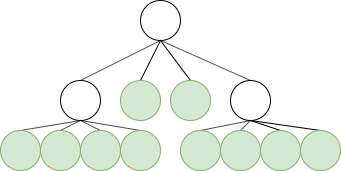
\includegraphics[scale=0.3]{2a.png}
        \end{itemize}        
      \end{itemize}
      \item For any $C \geq 0$ if $P(C)$ is true then $P(C + 1)$ must also be true.
      \begin{itemize}
        \item Assume that hypothesis for some value of $P(C)$ is true then we must show that $P(C + 1)$ is true.
        \item We can show this using the induction hpyothesis with an equation like so.
        \[(3C + 1) + 3(1) = 3(C + 1) + 1\]
        \item which using simple algebra is true.
      \end{itemize}
      \item Since steps 0 - 3 have been verified and we have shown that for every value if $P(C)$ is true then $P(C + 1)$ is true, therefore $L = 3C + 1$ for all natural number values of C.
    \end{itemize}

    \item \textbf{Proof by Induction}.
    \begin{enumerate}
      \item Conjecture. 
      \begin{lstlisting}
  def f(n):
    if n <= 0:
        return 4
    elif n <= 1:
        return 32
    else:
        return 8*f(n - 1) - 16*f(n - 2)

  print("f(0) = ", f(0))
  print("f(1) = ", f(1))
  print("f(2) = ", f(2))
  print("f(3) = ", f(3))

  #Output:
  f(0) =  4
  f(1) =  32
  f(2) =  192
  f(3) =  1024
      \end{lstlisting}

      Like the hint says lets look $4^n$. 

      \begin{lstlisting}
  print("4**0 = ", 4**0, ", diff = ", f(0) - 4**0, ", f(n)/4^n = ", f(0) / 4**0)
  print("4**1 = ", 4**1, ", diff = ", f(1) - 4**1, ", f(n)/4^n = ", f(1) / 4**1)
  print("4**2 = ", 4**2, ", diff = ", f(2) - 4**2, ", f(n)/4^n = ", f(2) / 4**2)
  print("4**3 = ", 4**3, ", diff = ", f(3) - 4**3, ", f(n)/4^n = ", f(3) / 4**3)
  print("4**4 = ", 4**4, ", diff = ", f(4) - 4**4, ", f(n)/4^n = ", f(4) / 4**4)
  print("4**5 = ", 4**5, ", diff = ", f(5) - 4**5, ", f(n)/4^n = ", f(5) / 4**5)

  #Output:
  4**0 =  1 , diff =  3 , f(n)/4^n =  4.0
  4**1 =  4 , diff =  28 , f(n)/4^n =  8.0
  4**2 =  16 , diff =  176 , f(n)/4^n =  12.0
  4**3 =  64 , diff =  960 , f(n)/4^n =  16.0
  4**4 =  256 , diff =  4864 , f(n)/4^n =  20.0
  4**5 =  1024 , diff =  23552 , f(n)/4^n =  24.0
      \end{lstlisting}

      Looking at the difference you can pretty easily see the difference between $4^n$ and $f(n)$ plus $4^n$ gives us $f(n + 1)$.
      
      Also if we look at $f(n) / 4^n$ we can see that $f(n) / 4^n = 4(n + 1)$.\\

      Therefore we can decude that \bm{$f(n) = 4^{(n + 1)}(n + 1)$}.
      
      \begin{lstlisting}
  def f2(n):
    return 4**(n + 1) * (n + 1)

  #Output:
  f(0) =  4 , f2(0) =  4
  f(1) =  32 , f2(1) =  32
  f(2) =  192 , f2(2) =  192
  f(3) =  1024 , f2(3) =  1024
  f(4) =  5120 , f2(4) =  5120
  f(5) =  24576 , f2(5) =  24576
      \end{lstlisting}

      \item Proof.   
   
      \begin{itemize}
        \item The Problem:
        \begin{itemize}
          \item We want to prove that the function $f(n)$ returns a value equilivent to the equation, $4^{(n + 1)}(n + 1)$.
          \item Given any natural number $n$.
        \end{itemize}
        \item The Inductive Steps:
        \begin{itemize}
          \item Base case $n = 0$. 
          \item True as $f(0) = 4$ and $4^1(1) = 4$
          \item Next step $n = 1$. 
          \item True as $f(1) = 32$ and $4^2(2) = 32$
          \item Next step $n = 2$. 
          \item True as $f(2) = 192$ and $4^3(3) = 192$
        \end{itemize}
        \item The Inductive Proof:
        \begin{itemize}
          \item Let's define our theory as for all $n > 0$ that if $P(n - 1)$ is true then $P(n)$ is also true. 
          \item If $n > 1$ then $f(n)$ returns $8*f(n - 1) - 16*f(n - 2)$. 
          \item However we know using the induction hypothesis that:          
          \item $f(n - 1)$ returns $4^n(n)$.
          \item And $f(n - 2)$ returns $4^{(n - 1)}(n - 1)$.
          \item Therefore we can say $f(n)$ returns:
          \item $8*(4^n(n)) - 16*(4^{(n - 1)}(n - 1))$.
          \item Which using algebra we can simplify that to $-4^{(1 + n)} (-1 + n) + 2^{(3 + 2 n)} n$.
          \item And even futher to an alternate form of $4^{(1 + n)} (1 + n)$.
          \item Which just so happens to be our target form.
        \end{itemize}
        \item Therefore we have proven using induction that given any natural number $n \geq 0$ that the function $f(n)$ returns a value equilivent to the equation, $4^{(n + 1)}(n + 1)$
      \end{itemize}
    \end{enumerate}

    \item \textbf{Graph Theory}.
    \begin{enumerate}
      \item Theory: Every free tree having at least two verticies has at least two verticies of degree 1.
      
      First lets define a Free Tree: An acyclic (containing no cycles), connected (no disconnected graphs, i.e. not a forest), unrooted (containing no special root node) graph.\\ 
      
      We want to prove that for every free tree that has $ verticies \geq 2$, they have $ verticies \geq 2$ of graph degree 1.\\

      If we start with the simplest case a free tree with two nodes, we can obvisouly see each node is connected to eachother so each node has a degree of one.\\

      Now lets think about what it means not to have any cycles in a tree that means we cannot have loops and adding any edge would create a cycle, therefore and using the theorm in graphs lecture \textbf{Number of edges = }\bm{$|E| = V - 1$} where V is the number of verticies in the tree.\\

      Next lets take our graph of $V$ verticies that means the max degree any one vertex can have is $V - 1$ and that every other node must have a degree of one because $E = V - 1$ as well, and the minimum degree any node can have is one otherwize it would not be connected, therefore there must be at least a subtree containing $v - 1$ nodes with v greater than two.\\ 

      That means no matter what you'll have leaf nodes that have 0 children and at most 1 degree of connection, and as we've already proven the base case of $n = 2$, any number of nodes greater than two will have at least two leaf nodes causing at least two nodes of degree one.

      \item Theory: Every connected, finite graph has at least one spanning subtree.\\
      
      A spanning subtree of a graph is a subtree that contains the minimum number of edges to contain all the verticies in the origional tree. This is equilivent to a free tree which has $V - 1$ edges which is the minimum you could have. \\
      
      A finite graph has a finite number of verticies $V$ and edges $E$.\\

      A connected graph means every pair of verticies has at least one connection or in other words there is at least one path from any two pairs of verticies.\\

      Therefore in a connected finite graph $G$ $|E| \geq V - 1$. And all you need to get the spanning subtree is remove edges until removing any additional edge disconnects $G$. 
      And due to the definiton of a connected graph there's at least one path from any node to another node so there must contain at least one path that connects all nodes which would give the spanning subtree.

      \item Theory: Every connected graph having at least two verticies has two distinct verticies that can be removed while staying a connected graph.

      We can apply an inductive reasoning to prove this:

      \begin{itemize}
        \item The problem.
        \begin{itemize}          
          \item $P(n) = $ Every connected graph having at least two verticies has two distinct verticies that can be removed while staying a connected graph.
        \end{itemize}
        \item The Inductive Steps.
        \begin{itemize}          
          \item Base case: $P(2) = $ A graph with two verticies if you remove both of them you have no graph which we'll assume is "connected" still. 
          \item $P(3)$ Remvoing any two verticies will leave a single vert which remains connected.
          \item $P(4)$ If one node has a degree of 3 you have three nodes you can remove, otherwise if you have two nodes with degree two you have those two nodes of degree one to remove.
          \item The Inductive case: Lets take a graph $G$ with $n + 1$ verticies. 
          \item Assume we'll attempt to remove one vertex $v$ giving us a new graph $G'$. 
          \item This gives us two possibilites.
          \item If the graph is still connected.
          \item Using the inductive hypothesis we know that $P(n)$ for all cases we proved about gave us at least two verticies we can remove therefore we'll get at least two more. 
          \item Otherwise if the graph gets disconnected by removing that node.
          \item If disconnected there must be at least two subgraphs created, $Sub_1, ... Sub_n$. 
          \item There is a vertex in each subgraph that was connected to $v$ or $v$ call it $v_x$.
          \item For each of the subgraphs we can recursively check them until we hit a case where we're still connected or a case case, thefore we have at two nodes we can remove eventually, however one of them must have been connected to the origional $v$ (or its recursions). 
          \item However we know that there are at least two original subgraphs thus giving us at least two nodes we'll find not connected in the origional graph $G$. 
        \end{itemize}
        \item Therefore we have proven every connected graph having at least two verticies has two distinct verticies that can be removed while staying a connected graph.
      \end{itemize}

      \item Theory: Given a graph having $n$ vertices and that for all vertices v in the graph, $deg(v) \geq n/2$.\\
      
      Base case: $P(1)$ a graph of one must be connected. $P(2)$ degree for each must equal $2/2$ therefore they must be connected to eachother.\\

      Now lets assume the our theory is incorrect that a graph can have two or more disconnected subgraphs. Each subgraph's nodes would still have to have $deg(v) \geq n/2$, thus each subgraph would need at least $\frac{n}{2} + 1$ vertices in them.
      That would make our total number of nodes for all subgraphs equal $(\frac{n}{2} + 1) + (\frac{n}{2} + 1) ...$ which would give us a total of $n + 2$ or more nodes which is impossible because our graph is defined as $n$ nodes.\\

      Therefore we have proven given a graph having $n$ vertices and that for all vertices v in the graph, $deg(v) \geq n/2$ because the alternative is impossible.\\

      An example of a graph where $deg(v) = n/2 -1$ for all v but is disconnected, would be our simple case of $P(2)$ each node would have a degree of $\frac{2}{2} - 1 = 0$ which is obvisouly just two stand alone disconnected nodes.
    \end{enumerate}

    \item \textbf{Huffman Trees and Binary Heaps}.
    
    \begin{enumerate}
      
      \item \textbf{Binary Heaps}
  
        Below is code that generates a list of 10,000 random numbers from range(0, 10000) and appends them to a file called Prob5aHeap.txt. 
        Then reads from that file to create an array of the integers, and out of that array builds a max binary heap. 
        Finally checks the heap to verify it is a valid heap.

        See in the zip file "Prob5aHeap.txt" for output and "Prob5aCheck.py" for code.

        \begin{lstlisting}
  import random
  import math     
  ı
  file_name = "Prob5aHeap.txt"

  def create_txt_file():
      f = open(file_name,"w+")
      for i in range(10000):
          f.write(str(random.randrange(10000)) + ",")
      f.close()
  
  def read_file():
      f = open(file_name, "r")
      txt = f.read()
      return [int(x) for x in txt.split(',') if x.strip().isdigit()]

      def build_max_heap(A, n):
      for i in range(parent(n), -1, -1): 
          max_heapify(A, i) 
  
  def max_heapify(A, i):    
      l = left(i)
      r = right(i)
      largest = i
  
      if l < len(A) and A[l] > A[i]:
          largest = l
      else:
          largest = i
          
      if r < len(A) and A[r] > A[largest]:
          largest = r
  
      if largest is not i:
          A[i], A[largest] = A[largest], A[i]        
          max_heapify(A, largest)
  
  def parent(i):
      return int((i / 2)) - 1
          
  def left(i):
      return 2 * i + 1
  
  def right(i):
      return (2 * i) + 2
  
  def is_heap(A, i): 
      if i > parent(i):  
          return True  
      
      if A[i] >= A[left(i)] and A[i] >= A[right(i)]:
          if is_heap(A, left(i)) and is_heap(A, right(i)):
              return True
        
      return False          
        \end{lstlisting}

        \begin{lstlisting}
  create_txt_file()
  A = read_file()     
  
  build_max_heap(A, len(A))
  is_heap(A, 0)
  
  # Output:
  # True

  f = open(file_name, "a+")
  f.write('\r\n\r\nResult:\r\n')
  f.write(str(A))
  f.close()      
        \end{lstlisting}


        \item \textbf{Huffman Trees}
        
        Below is the code to read in a file and scrub it of non ASCII characters.

        \begin{lstlisting}
  import random
  import math
  from matplotlib import pyplot as plt

  file_name = "Prob5b.txt"

  def read_file():
    f = open(file_name, "r")
    txt = f.read()
    txt = "".join(i for i in txt if ord(i) < 128)
    f.close()
    return txt
        \end{lstlisting}

        Next is code to compute the frequency distribution of the text and put them in a tuple of (frequcny, character).
        
        \begin{lstlisting}
  def build_freq_tups(A):
    f = {} 
    for c in A: 
        if (c in f): 
            f[c] += 1
        else: 
            f[c] = 1
            
    characters = f.keys()
    tuples = []
    for c in characters:
        tuples.append((f[c], c))    
    return tuples
        \end{lstlisting}
        
        Next is the code for this time converted to a min\_heap and the creation of the huffman tree.
        
        \begin{lstlisting}
  def huffman(C):
    Q = C
    while len(Q) > 1:
        left = extract_min(Q)
        right = extract_min(Q)
        freq = left[0] + right[0]
        insert(Q, (freq, (left, right)))
    return Q

  def build_min_heap(A, n):
    for i in range(parent(n), -1, -1): 
        min_heapify(A, i) 

  def min_heapify(A, i):    
    l = left(i)
    r = right(i)
    smallest = i

    if l < len(A) and A[l][0] < A[i][0]:
      smallest = l
    else:
      smallest = i
        
    if r < len(A) and A[r][0] < A[smallest][0]:
      smallest = r

    if smallest is not i:
      A[i], A[smallest] = A[smallest], A[i]        
      min_heapify(A, smallest)
        
  def extract_min(Q):
    x = Q[0]
    del Q[0]
    return x

  def insert(Q, z):
    Q.append(z)
    build_min_heap(Q, len(Q))

  def parent(i):
    return int((i / 2)) - 1
          
  def left(i):
    return 2 * i + 1

  def right(i):
    return (2 * i) + 2          
        \end{lstlisting}

        Also we have the code to create the codes from the huffman tree and to encode the text into its compessed form.

        \begin{lstlisting}
  def remove_freq(Q):
    p = Q[1]
    if type(p) == type(""):
      return p
    else: 
      return(remove_freq(p[0]), remove_freq(p[1]))

  def build_code_dict(node, code = '') :
    if type(node) == type(""):
      codes[node] = code
    else:
      build_code_dict(node[0], code + "0")
      build_code_dict(node[1], code + "1")
        
  def encode(text):
    encoded_str = ""
    for c in text:
        encoded_str += codes[c]
        
    f = open(file_name, "a+")
    f.write("\n\n" + encoded_str)
    f.close()
    return encoded_str   
        \end{lstlisting}

        Finally is the code that just calles these methods and puts the compressed text into the origional file.

        \begin{lstlisting}
  #Read file into an array of chars.
  text = read_file()
  A = [char for char in text] 
  
  #Print an example histogram.
  plt.hist(A)
  plt.title('Frequency Distribution')
  plt.xlabel('Character')
  plt.ylabel('Count')
  
  #Build the frequency table.
  F = build_freq_tups(A)
  
  #Create the huffman tree.
  Q = huffman(F)
  print(Q)
  
  #Build the code dictionary out of the huffman tree.
  codes = {}
  cleaned_Q = remove_freq(Q[0])
  code_dict = build_code_dict(cleaned_Q)
  print(codes)
  
  #Encode and compress the origional text.
  encoded_text = encode(text)
  print(encoded_text)          
        \end{lstlisting}

        Okay cool, so using all that if you look in Prob5b.txt we had an origional \textbf{character count of 10028 = (10028 * 8 bytes) = (80224 bits)} to our \textbf{encoded string of 43255 bits} which is a roughtly a \textbf{1:1.85} ratio of about half the size.\\

        Please refer to Prob5bHuff.py for the code and Prob5b.txt for the text and compessed text.

  \end{enumerate}

  \item \textbf{Heap Comparisons}

  \end{enumerate}  % End of questions.
\end{document}
